\documentclass[a4paper]{article}
\usepackage[a4paper,margin=0mm]{geometry}
\usepackage{fontspec}
\usepackage{unicode-math}
\usepackage{tikz}
\usepackage[table]{xcolor}
\usepackage[absolute]{textpos}
\usepackage{enumitem}
\usepackage{array}
\usepackage{multirow}

\setmainfont{Libertinus Serif}
\setsansfont{Libertinus Sans}
\setmathfont{Libertinus Math}
\newfontfamily\trackedsans{Libertinus Sans}[LetterSpace=8.0]

\definecolor{accent}{HTML}{F46530}
\definecolor{badge}{HTML}{FFBDA5}
\definecolor{ink}{HTML}{2A2E30}

\setlength{\TPHorizModule}{1mm}
\setlength{\TPVertModule}{1mm}
\setlength{\parindent}{0pt}
\pagestyle{empty}

\newcommand{\LCOL}{16mm}
\newcommand{\RCOL}{111mm}
\newcommand{\COLW}{83mm}

\newcommand{\topicheader}[2]{%
\begin{textblock*}{194mm}(16mm,10mm)
\begin{tikzpicture}
\node[fill=accent,text=white,font=\sffamily\bfseries\fontsize{13}{13}\selectfont,
      minimum width=9mm,minimum height=9mm,inner sep=0pt] at (4.5mm,-4.5mm) {#1};
\node[font=\sffamily\bfseries\fontsize{15}{16}\selectfont,text=ink,anchor=west] at (12mm,-4.5mm) {#2};
\end{tikzpicture}
\end{textblock*}
\begin{textblock*}{194mm}(16mm,22.5mm)

\begin{tikzpicture}
\fill[accent] (0,0) rectangle (194mm,0.5mm);
\end{tikzpicture}
\end{textblock*}
}

\newcommand{\pagefooter}[1]{%
\begin{textblock*}{194mm}(8mm,286.41mm)
  
\begin{tikzpicture}
    \fill[accent] (0,0) rectangle (194mm,0.6mm);
  \end{tikzpicture}
\end{textblock*}
\begin{textblock*}{63.59mm}(8mm,288.27mm)
  {\sffamily\bfseries\color{accent}\fontsize{13}{16}\selectfont SAT 1200+}
\end{textblock*}
\begin{textblock*}{10mm}(188mm,288.27mm)
  \centering{\sffamily\color{accent}\fontsize{14}{16}\selectfont #1}
\end{textblock*}
}

\newcommand{\colrule}[2]{%
\begin{textblock*}{1mm}(105mm,#1mm)
\begin{tikzpicture}
\draw[black!65,line width=0.5pt] (0,0) -- (0,#2mm);
\end{tikzpicture}
\end{textblock*}
}

\newcommand{\setkicker}[2]{%
{\sffamily\bfseries\fontsize{12}{14}\selectfont #1.}\ {\itshape\fontsize{11}{14}\selectfont\color{black!75} #2}\par\vspace{2mm}%
}

\setlength{\fboxsep}{1.4pt}
\setlength{\fboxrule}{0.5pt}
\newcommand{\pnum}[1]{\fcolorbox{ink}{white}{\sffamily\bfseries\fontsize{8}{8}\selectfont #1}~}

\newcommand{\qrbox}[1]{%
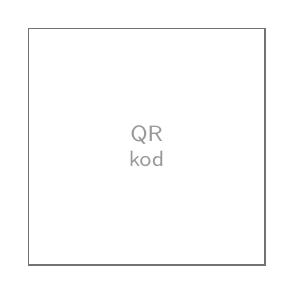
\begin{tikzpicture}
\draw[black!55,line width=0.6pt] (0,0) rectangle (30mm,30mm);
\node[black!40,font=\sffamily\fontsize{8}{9}\selectfont,align=center] at (15mm,15mm) {QR\\kod};
\end{tikzpicture}\\[1.5mm]
{\sffamily\fontsize{9}{11}\selectfont\color{black!70} #1}%
}

% ---- SAT-style multiple-choice question block: #1=number #2=stem #3-6=choices A-D ----
\newcommand{\satq}[6]{%
\noindent\pnum{#1} #2\\[2mm]
\hspace*{7mm}\begin{tabular}{@{}p{32mm}p{32mm}@{}}
(A) #3 & (B) #4 \\[2.5mm]
(C) #5 & (D) #6 \\
\end{tabular}\\[7mm]%
}

\arrayrulecolor{accent}
\setlength{\arrayrulewidth}{0.7pt}
\renewcommand{\arraystretch}{1.35}
\newcommand{\anstitle}[1]{{\sffamily\bfseries\color{accent}\fontsize{11}{13}\selectfont #1}\\[1.3mm]}

\begin{document}

% ================= PAGE 1: Set 1 | Set 2 =================
\topicheader{8}{Koordinata tekisligi va funksiya}
\pagefooter{52}
\colrule{32}{238}
\mbox{}%

\begin{textblock*}{\COLW}(\LCOL,32mm)
{\fontsize{12}{15}\selectfont
\setkicker{1-to'plam}{Nuqta qaysi chorakka tegishli ekanini aniqlang.}

\noindent\pnum{1} $(3,\ 5)\ \to$ chorak:\\[22mm]
\noindent\pnum{2} $(-2,\ 4)\ \to$ chorak:\\[22mm]
\noindent\pnum{3} $(-6,\ -1)\ \to$ chorak:\\[22mm]
\noindent\pnum{4} $(7,\ -3)\ \to$ chorak:\\[22mm]
\noindent\pnum{5} $(-4,\ -8)\ \to$ chorak:\\[22mm]
\noindent\pnum{6} $(5,\ -5)\ \to$ chorak:\\[22mm]
\noindent\pnum{7} $(-9,\ 2)\ \to$ chorak:\\[22mm]
\noindent\pnum{8} $(1,\ 1)\ \to$ chorak:
}
\end{textblock*}

\begin{textblock*}{\COLW}(\RCOL,32mm)
{\fontsize{12}{15}\selectfont
\setkicker{2-to'plam}{Tenglamadan $k$ (burchak koeffitsienti) va $b$ ni ajrating.}

\noindent\pnum{1} $y=3x+7\ \to k{=}\;\;b{=}$\\[22mm]
\noindent\pnum{2} $y=-2x+1\ \to k{=}\;\;b{=}$\\[22mm]
\noindent\pnum{3} $y=x-5\ \to k{=}\;\;b{=}$\\[22mm]
\noindent\pnum{4} $y=-x+9\ \to k{=}\;\;b{=}$\\[22mm]
\noindent\pnum{5} $y=4x\ \to k{=}\;\;b{=}$\\[22mm]
\noindent\pnum{6} $y=-6\ \to k{=}\;\;b{=}$\\[22mm]
\noindent\pnum{7} $y=0.5x-3\ \to k{=}\;\;b{=}$\\[22mm]
\noindent\pnum{8} $y=\dfrac{1}{3}x-2\ \to k{=}\;\;b{=}$
}
\end{textblock*}

\clearpage

% ================= PAGE 2: Set 3 | Set 4 =================
\topicheader{8}{Koordinata tekisligi va funksiya}
\pagefooter{53}
\colrule{32}{238}
\mbox{}%

\begin{textblock*}{\COLW}(\LCOL,32mm)
{\fontsize{12}{15}\selectfont
\setkicker{3-to'plam}{$f(a)$ ni musbat qiymatlar uchun hisoblang.}

\noindent\pnum{1} $f(x)=2x+3$. $f(4)=$\\[22mm]
\noindent\pnum{2} $f(x)=5x-1$. $f(2)=$\\[22mm]
\noindent\pnum{3} $f(x)=-3x+4$. $f(1)=$\\[22mm]
\noindent\pnum{4} $f(x)=x+10$. $f(0)=$\\[22mm]
\noindent\pnum{5} $f(x)=4x$. $f(3)=$\\[22mm]
\noindent\pnum{6} $f(x)=-x+6$. $f(5)=$\\[22mm]
\noindent\pnum{7} $f(x)=2x-7$. $f(10)=$\\[22mm]
\noindent\pnum{8} $f(x)=-5x+2$. $f(3)=$
}
\end{textblock*}

\begin{textblock*}{\COLW}(\RCOL,32mm)
{\fontsize{12}{15}\selectfont
\setkicker{4-to'plam}{$f(a)$ ni manfiy qiymatlar uchun hisoblang -- manfiy son har doim qavsda.}

\noindent\pnum{1} $f(x)=3x+2$. $f(-2)=$\\[22mm]
\noindent\pnum{2} $f(x)=-4x+1$. $f(-3)=$\\[22mm]
\noindent\pnum{3} $f(x)=x+8$. $f(-8)=$\\[22mm]
\noindent\pnum{4} $f(x)=x^2$. $f(-3)=$\\[22mm]
\noindent\pnum{5} $f(x)=x^2+1$. $f(-4)=$\\[22mm]
\noindent\pnum{6} $f(x)=2x^2-3$. $f(-2)=$\\[22mm]
\noindent\pnum{7} $f(x)=-x^2$. $f(-5)=$\\[22mm]
\noindent\pnum{8} $f(x)=(x+1)^2$. $f(-6)=$
}
\end{textblock*}

\clearpage

% ================= PAGE 3: Set 5 | Set 6 (spot the error) =================
\topicheader{8}{Koordinata tekisligi va funksiya}
\pagefooter{54}
\colrule{32}{238}
\mbox{}%

\begin{textblock*}{\COLW}(\LCOL,32mm)
{\fontsize{11}{14}\selectfont
\setkicker{5-to'plam}{Aralash -- shaklni almashtiring, qiymatni hisoblang, tenglamani yeching.}

\noindent\pnum{1} $y=5x-3$ ni $f(x)$ shaklida yozing va $f(2)$ ni toping.\\[14mm]
\noindent\pnum{2} $f(x)=-2x+8$ ni $y=kx+b$ shaklida yozing, $k,b$ ni toping.\\[14mm]
\noindent\pnum{3} $y=x+1$ ni $f(x)$ shaklida yozing, so'ng $f(-4)$ ni hisoblang.\\[14mm]
\noindent\pnum{4} $f(x)=4x-9$. Agar $f(x)=11$ bo'lsa, $x$ ni toping.\\[14mm]
\noindent\pnum{5} $f(x)=-3x+6$. Agar $f(x)=0$ bo'lsa, $x$ ni toping.\\[14mm]
\noindent\pnum{6} $y=-x-5$ ni $f(x)$ shaklida yozing va $f(0)$ ni toping.\\[14mm]
\noindent\pnum{7} $f(x)=2x+1$ bo'lsa, $f(3)+f(-3)$ ni hisoblang.\\[14mm]
\noindent\pnum{8} $f(x)=x^2-4$. Agar $f(a)=5$ bo'lsa, $a$ ning musbat qiymatini toping.
}
\end{textblock*}

\begin{textblock*}{\COLW}(\RCOL,32mm)
{\fontsize{10.5}{13}\selectfont
\setkicker{6-to'plam}{Xatoni toping -- buzilgan qadamni ayting, to'g'ri javobni bering.}

\noindent\pnum{1} $f(x)=3x+2$. $f(5)$ ni toping:\\[1mm]
\hspace*{7mm}\textit{``$f(5)=f\cdot5$, $f$ noma'lum, javob topib bo'lmaydi.''}\\[2mm]
\hspace*{7mm}Xato va to'g'ri javob: \makebox[52mm]{\dotfill}\\[6mm]

\noindent\pnum{2} $f(x)=x^2$. $f(-4)$ ni toping:\\[1mm]
\hspace*{7mm}\textit{``$f(-4)=-4^2=-16$.''}\\[2mm]
\hspace*{7mm}Xato va to'g'ri javob: \makebox[52mm]{\dotfill}\\[6mm]

\noindent\pnum{3} $(-3,\ 5)$ nuqtasi qaysi chorakda?\\[1mm]
\hspace*{7mm}\textit{``$x=-3$ ni musbat deb o'ylab, I chorak.''}\\[2mm]
\hspace*{7mm}Xato va to'g'ri javob: \makebox[52mm]{\dotfill}\\[6mm]

\noindent\pnum{4} $f(x)=2x-5$. Agar $f(x)=7$, $x$ ni toping:\\[1mm]
\hspace*{7mm}\textit{``$2x-5=7\Rightarrow2x=2\Rightarrow x=1$.''}\\[2mm]
\hspace*{7mm}Xato va to'g'ri javob: \makebox[52mm]{\dotfill}\\[6mm]

\noindent\pnum{5} $f(x)=x^2+3$. $f(-2)$ ni toping:\\[1mm]
\hspace*{7mm}\textit{``$f(-2)=-2^2+3=-4+3=-1$.''}\\[2mm]
\hspace*{7mm}Xato va to'g'ri javob: \makebox[52mm]{\dotfill}
}
\end{textblock*}

\clearpage

% ================= PAGE 4: Set 7 (bonus) -- own page =================
\topicheader{8}{Koordinata tekisligi va funksiya}
\pagefooter{55}
\colrule{32}{238}
\mbox{}%

\begin{textblock*}{\COLW}(\LCOL,32mm)
{\fontsize{12}{15}\selectfont
\setkicker{7-to'plam}{Bonus / qiyin -- har biriga taxminan 90 soniya.}

\noindent\pnum{1} $f(x)=2x^2-3x+1$. $f(-2)=$\\[26mm]
\noindent\pnum{2} $f(x)=-(x-3)^2$. $f(6)=$\\[26mm]
\noindent\pnum{3} $y=-4x+11$ ni $f(x)$ shaklida yozing, so'ng $f(x)=3$ bo'lganda $x$ ni toping.\\[26mm]
\noindent\pnum{4} $f(x)=x^2-2x$. Agar $f(a)=8$ bo'lsa, $a$ ning manfiy qiymatini toping.\\[26mm]
\noindent\pnum{5} $f(x)=3x+c$. Agar $f(2)=10$ bo'lsa, $c$ ni toping.
}
\end{textblock*}

\clearpage

% ================= PAGE 5: Set 8 (SAT-style application, MC) -- own page =================
\topicheader{8}{Koordinata tekisligi va funksiya}
\pagefooter{56}
\colrule{32}{238}
\mbox{}%

\begin{textblock*}{\COLW}(\LCOL,32mm)
{\fontsize{10.5}{13}\selectfont
\setkicker{8-to'plam}{SAT'da qanday uchraydi -- chorak, qiyalik va funksiya qiymati.}

\satq{1}{$(-5,\ 3)$ nuqtasi qaysi chorakda joylashgan?}{II}{I}{III}{IV}
\satq{2}{$y=-2x+9$ to'g'ri chizig'ining qiyaligi ($k$) nechaga teng?}{2}{$-2$}{9}{$-9$}
\satq{3}{$y=7x-4$ to'g'ri chizig'ining erkin hadi ($b$) nechaga teng?}{7}{4}{$-4$}{$-7$}
\satq{4}{Agar $f(x)=3x-5$ bo'lsa, $f(4)$ nechaga teng?}{12}{17}{$-5$}{7}
\satq{5}{Agar $f(x)=x^2+2$ bo'lsa, $f(-3)$ nechaga teng?}{11}{$-7$}{7}{$-11$}
\satq{6}{$(0,\ -6)$ nuqtadan o'tuvchi va qiyaligi $4$ ga teng bo'lgan chiziq tenglamasi qaysi?}{$y{=}{-}6x{+}4$}{$y{=}4x{-}6$}{$y{=}4x{+}6$}{$y{=}{-}4x{-}6$}
}
\end{textblock*}

\begin{textblock*}{\COLW}(\RCOL,32mm)
{\fontsize{10.5}{13}\selectfont
\vspace{9mm}

\satq{7}{$(6,\ -2)$ nuqtasi qaysi chorakda joylashgan?}{I}{II}{IV}{III}
\satq{8}{$y=-x+3$ to'g'ri chizig'i Oy o'qini qaysi nuqtada kesib o'tadi?}{$(3,0)$}{$(0,-1)$}{$(-1,0)$}{$(0,3)$}
\satq{9}{Agar $g(x)=2x+1$ bo'lsa, $g(5)-g(1)$ nechaga teng?}{8}{4}{14}{2}
\satq{10}{$y=\dfrac{1}{2}x-4$ to'g'ri chizig'ining qiyaligi ($k$) nechaga teng?}{$-4$}{$\frac12$}{2}{$-\frac12$}
\satq{11}{Agar $h(x)=-x^2+4$ bo'lsa, $h(-2)$ nechaga teng?}{8}{$-4$}{0}{4}
\satq{12}{$y=3x-2$ to'g'ri chizig'ida qaysi nuqta yotadi?}{$(2,6)$}{$(4,2)$}{$(2,-4)$}{$(2,4)$}
}
\end{textblock*}

\clearpage

% ================= PAGE 6: Javoblar -- unified answer table =================
\topicheader{8}{Koordinata tekisligi va funksiya}
\pagefooter{57}
\mbox{}%

\begin{textblock*}{194mm}(16mm,30mm)
{\bfseries\itshape\color{accent}\fontsize{19}{21}\selectfont\centering Javoblar\par}
\end{textblock*}

\begin{textblock*}{194mm}(16mm,44mm)
{\fontsize{9.5}{12}\selectfont
\centering
\renewcommand{\arraystretch}{1.3}
\begin{tabular}{|>{\centering\arraybackslash}p{24mm}|>{\centering\arraybackslash}p{9mm}|>{\centering\arraybackslash}p{30mm}|>{\centering\arraybackslash}p{9mm}|>{\centering\arraybackslash}p{30mm}|}
\hline
\rowcolor{badge!55}\textbf{To'plam} & \textbf{\#} & \textbf{Javob} & \textbf{\#} & \textbf{Javob}\\
\hline
\multirow{4}{24mm}{\centering 1-to'plam} & 1 & I & 2 & II\\\cline{2-5}
 & 3 & III & 4 & IV\\\cline{2-5}
 & 5 & III & 6 & IV\\\cline{2-5}
 & 7 & II & 8 & I\\\hline
\multirow{4}{24mm}{\centering 2-to'plam} & 1 & $k{=}3,b{=}7$ & 2 & $k{=}{-}2,b{=}1$\\\cline{2-5}
 & 3 & $k{=}1,b{=}{-}5$ & 4 & $k{=}{-}1,b{=}9$\\\cline{2-5}
 & 5 & $k{=}4,b{=}0$ & 6 & $k{=}0,b{=}{-}6$\\\cline{2-5}
 & 7 & $k{=}0.5,b{=}{-}3$ & 8 & $k{=}\frac13,b{=}{-}2$\\\hline
\multirow{4}{24mm}{\centering 3-to'plam} & 1 & 11 & 2 & 9\\\cline{2-5}
 & 3 & 1 & 4 & 10\\\cline{2-5}
 & 5 & 12 & 6 & 1\\\cline{2-5}
 & 7 & 13 & 8 & $-13$\\\hline
\multirow{4}{24mm}{\centering 4-to'plam} & 1 & $-4$ & 2 & 13\\\cline{2-5}
 & 3 & 0 & 4 & 9\\\cline{2-5}
 & 5 & 17 & 6 & 5\\\cline{2-5}
 & 7 & $-25$ & 8 & 25\\\hline
\multirow{5}{24mm}{\centering 5-to'plam} & \multicolumn{4}{p{78mm}|}{1.\ $f(x)=5x-3$; $f(2)=7$ \quad\quad 2.\ $y=-2x+8$; $k=-2,\,b=8$}\\\cline{2-5}
 & \multicolumn{4}{p{78mm}|}{3.\ $f(x)=x+1$; $f(-4)=-3$ \quad\quad 4.\ $x=5$}\\\cline{2-5}
 & \multicolumn{4}{p{78mm}|}{5.\ $x=2$ \quad\quad 6.\ $f(x)=-x-5$; $f(0)=-5$}\\\cline{2-5}
 & \multicolumn{4}{p{78mm}|}{7.\ $f(3)+f(-3)=7+(-5)=2$}\\\cline{2-5}
 & \multicolumn{4}{p{78mm}|}{8.\ $a=3$}\\\hline
\multirow{3}{24mm}{\centering 7-to'plam} & 1 & 15 & 2 & $-9$\\\cline{2-5}
 & \multicolumn{4}{p{78mm}|}{3.\ $f(x)=-4x+11$; $x=2$ \quad 4.\ $a=-2$ \quad 5.\ $c=4$}\\\hline
\multirow{6}{24mm}{\centering 8-to'plam} & 1 & A & 2 & B\\\cline{2-5}
 & 3 & C & 4 & D\\\cline{2-5}
 & 5 & A & 6 & B\\\cline{2-5}
 & 7 & C & 8 & D\\\cline{2-5}
 & 9 & A & 10 & B\\\cline{2-5}
 & 11 & C & 12 & D\\\hline
\multirow{5}{24mm}{\centering 6-to'plam} & \multicolumn{4}{p{78mm}|}{1.\ $f$ funksiya nomi, songa ko'paytirilmaydi. To'g'ri: $f(5)=3(5)+2=17$.}\\\cline{2-5}
 & \multicolumn{4}{p{78mm}|}{2.\ Manfiy kiritmada qavs tushib qolgan. To'g'ri: $f(-4)=(-4)^2=16$.}\\\cline{2-5}
 & \multicolumn{4}{p{78mm}|}{3.\ $x$ ning ishorasi noto'g'ri o'qilgan. To'g'ri: $x{=}-3{<}0,y{=}5{>}0\Rightarrow$ II chorak.}\\\cline{2-5}
 & \multicolumn{4}{p{78mm}|}{4.\ $7+5=12$, $2$ emas. To'g'ri: $2x=12\Rightarrow x=6$.}\\\cline{2-5}
 & \multicolumn{4}{p{78mm}|}{5.\ Yana qavs tushib qolgan. To'g'ri: $f(-2)=(-2)^2+3=7$.}\\\hline
\end{tabular}
}
\end{textblock*}

\begin{textblock*}{194mm}(16mm,240mm)
\centering
{\sffamily\fontsize{9.5}{11.5}\selectfont\color{black!70} Video yechimlar va qo'shimcha testlar uchun quyidagi QR kodlarni skanerlang:}\\[4mm]
\begin{minipage}[t]{32mm}\centering\qrbox{YouTube}\end{minipage}%
\hspace{16mm}%
\begin{minipage}[t]{32mm}\centering\qrbox{Telegram}\end{minipage}
\end{textblock*}

\end{document}
